\documentclass[tikz, border=5mm]{standalone}
\usetikzlibrary{positioning, arrows.meta, calc, fit, backgrounds}

\begin{document}
	
	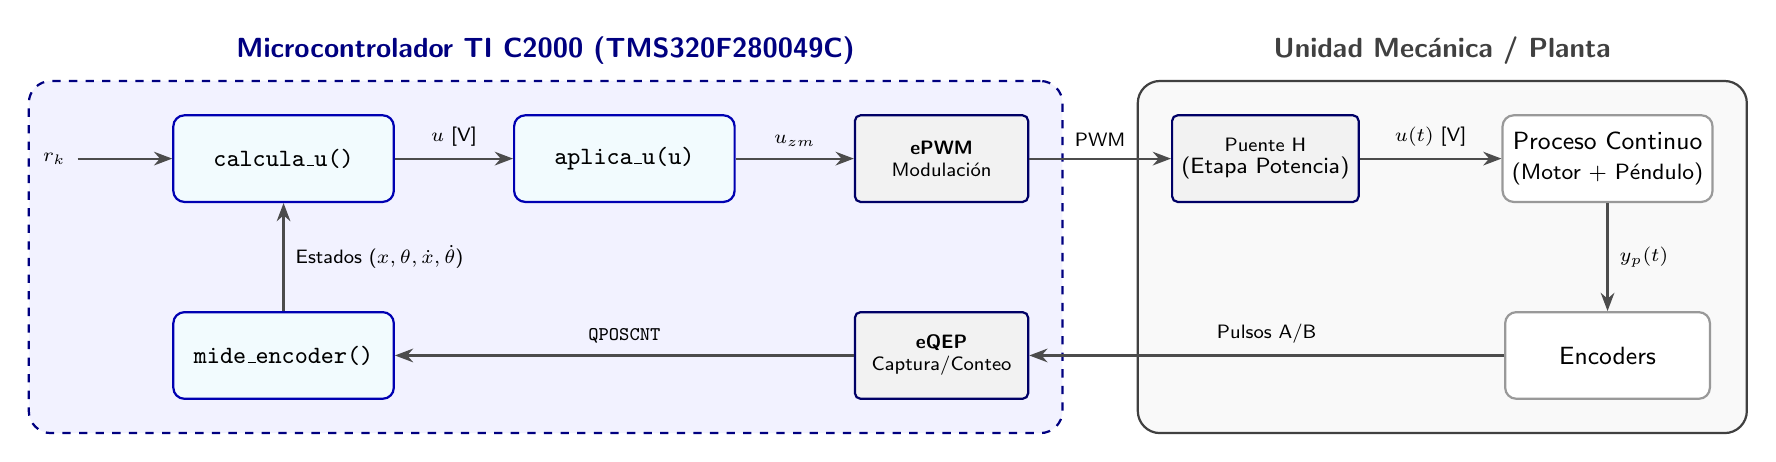
\begin{tikzpicture}[
		% Separación global regulada
		node distance=1.5cm and 1.8cm,
		% Estilos diferenciados: Software vs Hardware
		software/.style={draw=blue!70!black, fill=cyan!5, thick, rectangle, rounded corners=4pt, minimum height=1.1cm, minimum width=2.8cm, align=center, font=\sffamily\small},
		periferico/.style={draw=blue!40!black, fill=gray!10, thick, rectangle, rounded corners=2pt, minimum height=1.1cm, minimum width=2.2cm, align=center, font=\sffamily\scriptsize},
		hardware/.style={draw=gray!80, fill=white, thick, rectangle, rounded corners=4pt, minimum height=1.1cm, minimum width=2.6cm, align=center, font=\sffamily\small},
		% Estilo de cajas de entorno
		mcu_box/.style={draw=blue!50!black, fill=blue!5, thick, rounded corners=8pt, dashed},
		planta_box/.style={draw=gray!50!black, fill=gray!5, thick, rounded corners=8pt},
		% Estilo de flechas y etiquetas
		flecha/.style={-{Stealth[scale=1.0]}, thick, draw=black!70},
		label_est/.style={font=\scriptsize\sffamily, fill=none, inner sep=4pt}
		]
		
		% --- ENTORNO ENTRADA ---
		% Nodo virtual de referencia para alinear la consigna de entrada
		\coordinate (origen_r) at (-2.0, 2.2);
		
		% --- CAPA DEL MICROCONTROLADOR (Firmware y Periféricos) ---
		% Fila Superior (Cálculo y Actuación)
		\node[software] (control) at (0, 2.2) {\textbf{\texttt{calcula\_u()}}};
		\node[software, right=1.5cm of control] (aplica) {\textbf{\texttt{aplica\_u(u)}}};
		\node[periferico, right=1.5cm of aplica] (pwm) {\textbf{ePWM} \\ Modulación};
		
		% Fila Inferior (Adquisición y Captura)
		\node[periferico] (eqep) at ($(pwm)-(0, 2.5)$) {\textbf{eQEP} \\ Captura/Conteo};
		\node[software, at={(control |- eqep)}] (mide) {\textbf{\texttt{mide\_encoder()}}};
		
		% Flecha de consigna de entrada r_k
		\draw[flecha] ($(control.west)-(1.2,0)$) -- (control.west) node[label_est, pos=0, left, black] {$r_k$};
		
		% --- CAPA DE HARDWARE EXTERNO (Derecha) ---
		\node[periferico, right=1.8cm of pwm] (driver) {Puente H \\ \footnotesize (Etapa Potencia)};
		\node[hardware, right=1.8cm of driver] (proceso) {Proceso Continuo \\ \footnotesize (Motor + Péndulo)};
		\node[hardware, at={(proceso |- eqep)}] (sensor) {Encoders};
		
		% --- CONEXIONES DEL LAZO CERRADO (Flujo Secuencial) ---
		% 1. Adquisición hacia el cálculo
		\draw[flecha] (eqep) -- node[label_est, above] {\textbf{\texttt{QPOSCNT}}} (mide);
		\draw[flecha] (mide) -- node[label_est, right] {Estados ($x, \theta, \dot{x}, \dot{\theta}$)} (control);
		
		% 2. Cálculo hacia la periferia de salida
		\draw[flecha] (control) -- node[label_est, above] {$u$ [V]} (aplica);
		\draw[flecha] (aplica) -- node[label_est, above] {$u_{zm}$} (pwm);
		
		% 3. Salida hacia el hardware externo
		\draw[flecha] (pwm) -- node[label_est, above] {PWM} (driver);
		\draw[flecha] (driver) -- node[label_est, above] {$u(t)$ [V]} (proceso);
		
		% 4. Retorno del proceso hacia los sensores y capturadores
		\draw[flecha] (proceso) -- node[label_est, right] {$y_p(t)$} (sensor);
		\draw[flecha] (sensor) -- node[label_est, above] {Pulsos A/B} (eqep);
		
		% --- CAJAS DE FONDO REORGANIZADAS ---
		\begin{scope}[on background layer]
			% Envoltura síncrona del Microcontrolador
			\node[mcu_box, fit={(control) (aplica) (pwm) (eqep) (mide) ($(control.west)-(1.4,0)$)}, inner sep=12pt] (mcu) {};
			\node[above=2pt of mcu.north, font=\sffamily\bfseries\color{blue!50!black}] {Microcontrolador TI C2000 (TMS320F280049C)};
			
			% Envoltura de la planta física externa
			\node[planta_box, fit={(driver) (proceso) (sensor)}, inner sep=12pt] (planta) {};
			\node[above=2pt of planta.north, font=\sffamily\bfseries\color{gray!50!black}] {Unidad Mecánica / Planta};
		\end{scope}
		
	\end{tikzpicture}
	
\end{document}